\documentclass{fhnwreport} %
\usepackage[ngerman]{babel}
\usepackage[T1]{fontenc}
\usepackage[utf8]{inputenc}
\usepackage{tikz}
\usepackage{amsmath}
\usetikzlibrary{arrows}
\usepackage{lmodern}      % Type1-Schriftart für nicht-englische Texte 
\usepackage{subfigure}
\usepackage{listings}
\usepackage{color}
\usepackage{graphicx}
\usepackage{varwidth}
\usepackage{mwe}


\definecolor{dkgreen}{rgb}{0,0.6,0}
\definecolor{gray}{rgb}{0.5,0.5,0.5}
\definecolor{mauve}{rgb}{0.58,0,0.82}

\lstset{frame=tb,
  language=Python,
  aboveskip=3mm,
  belowskip=3mm,
  showstringspaces=false,
  columns=flexible,
  basicstyle={\small\ttfamily},
  numbers=none,
  numberstyle=\tiny\color{gray},
  keywordstyle=\color{blue},
  commentstyle=\color{dkgreen},
  stringstyle=\color{mauve},
  breaklines=true,
  breakatwhitespace=true,
  tabsize=3
}

%%% Harvard-Style Bibliographie
%\usepackage{natbib}
%\bibliographystyle{agsm}

%%% IEEE-Style Bibliographie
\bibliographystyle{IEEEtran}

%% Und wenn die Bibliographie im Inhaltsverzeichnis sein soll:
\usepackage[nottoc]{tocbibind}


\title{%
  {\huge Das bestimmte Integral und seine Anwendungen}\\[2ex]
  {\large Semesterarbeit Einführung in die Analysis (eana)}}
\author{Florian Thiévent}

\begin{document}

% Titel
\maketitle

\vfill

% Titelbild
% (kann man natürlich auch mit Includegraphics machen)
\begin{minipage}{\textwidth}
\begin{center}
\vspace*{5ex}
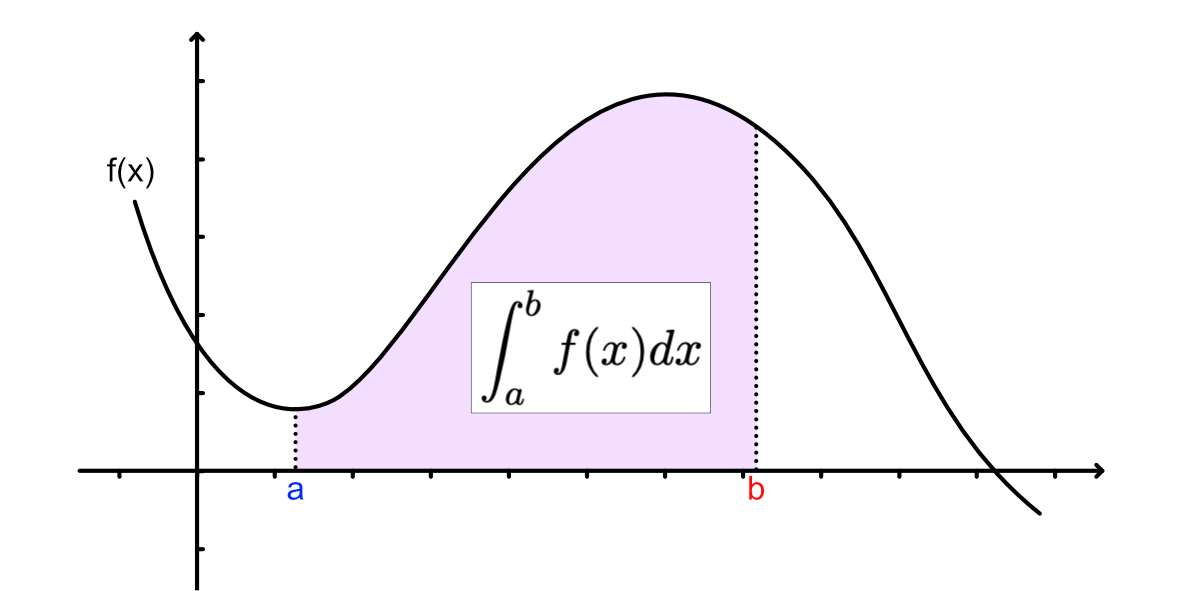
\includegraphics{titelbild}
\end{center}
\end{minipage}

\vfill

\begin{tabbing}
Dozent: \hspace{2em} \= Andreas Leiser \\[2ex]
Studiengang: \> Informatik
\end{tabbing}


\hbox{}

\clearpage

% Inhaltsverzeichnis
\tableofcontents
\clearpage

%\cite{Bosch2010}}
\section{Motivierung}
Die Integralrechnung stellt die Umkehrung der Differentialrechnung dar \cite{Bosch2010}. Dabei wird zwischen dem unbestimmten und dem bestimmten Integral unterschieden. Im Unterschied zum unbestimmten Integral kann mit dem bestimmten Integral ein konkreter Zahlenwert berechnet werden. Ob es sich um ein unbestimmtes oder bestimmtes Integral handelt, wird durch das Vorhandensein von Integrationsgrenzen bestimmt. Das bestimmte Integral kann dazu verwendet werden, den Flächeninhalt zwischen einem Graphen und der Koordinatenachse oder zwischen zwei Graphen zu berechnen. In dieser Arbeit wird das Riemann'sche Integral verwendet, um das bestimmte Integral zwischen dem Graphen einer Funktion und einer Koordinatenachse zu berechnen. Es wird der Unterschiede zwischen dem Vorgehen mit der Riemann'schen Summe und der Darboux Methode gezeigt.

\clearpage
% Abschnitt fertig

\section{Theorie: Das bestimmte Integral}
\subsection{Allgemeines}
Mit dem bestimmten Integral kann der Flächeninhalt unter einer Funktion $f$ über einem bestimmten Intervall auf der $x$-Achse berechnet werden. Man erhält für nichtnegative Funktionen bei Kurven oberhalb der $x$-Achse den positiven Flächeninhalt und bei Kurven unterhalb der $x$-Achse den negativen Flächeninhalt. 

\begin{figure*}[!h]
\centering
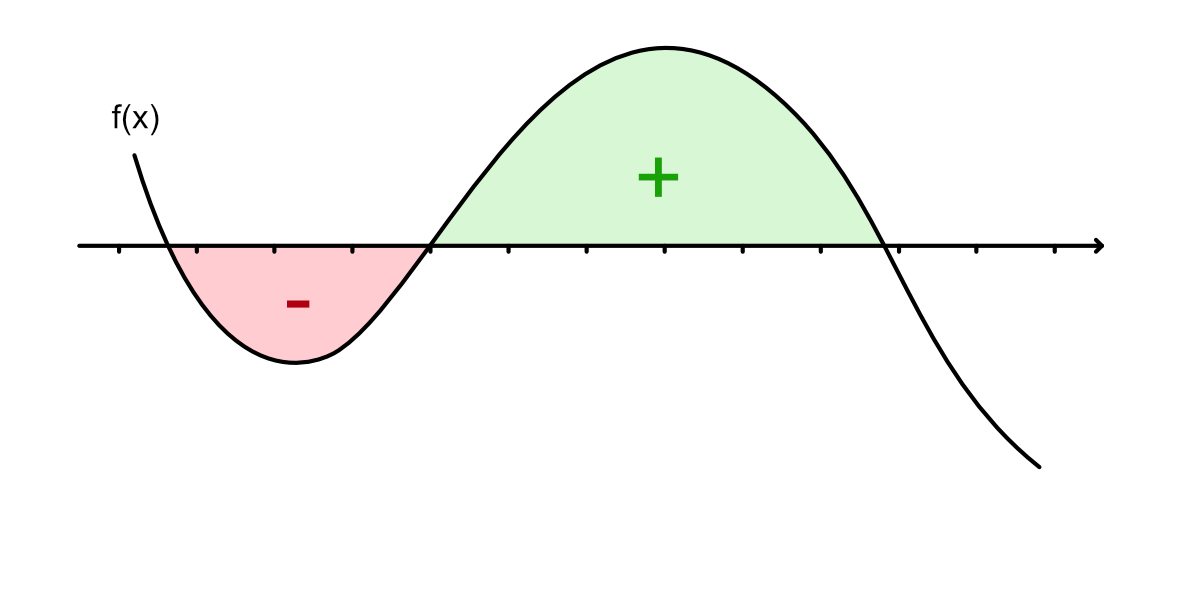
\includegraphics{orientierte-flaeche}
\caption{Orientierte Fläche}
\label{fig:orientierte_flaeche}
\end{figure*}


Der zu berechnende Flächeninhalt wird durch Integrationsgrenzen festgelegt. Der Abschnitt zwischen den Integrationsgrenzen wird Intervall genannt. 

\begin{figure*}[!h]
\centering
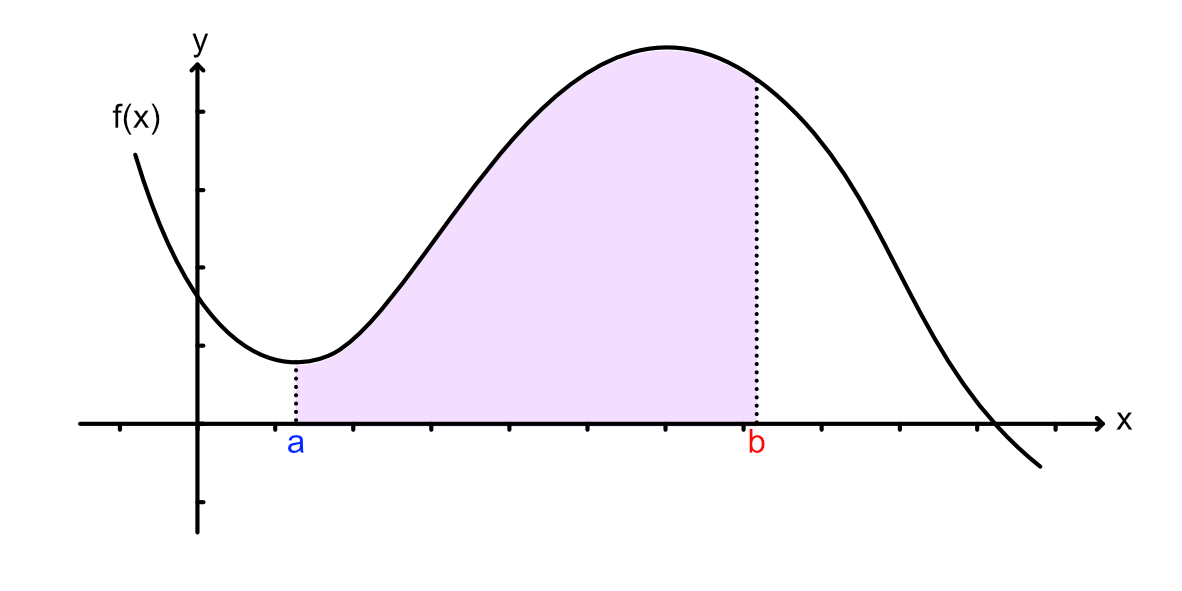
\includegraphics{flaecheninhalt}
\caption{Zu berechnender Flächeninhalt (violett) mit Intervall [a,b]}
\label{fig:flaecheninhalt_violett}
\end{figure*}

\subsubsection{Vorgehen nach Riemann}
Die Herausforderung bei der Berechnung von Flächeninhalten unter einem Graphen ist, dass es keine "Formel" gibt wie man diese aus der Geometrie kennt, um beispielsweise Flächen von Rechtecken, Dreiecken oder Quadraten zu berechnen. Es ist jedoch möglich, dieses Wissen zu nutzen, um eine Näherung zu erhalten. Die zu berechnende Fläche des Intervalls wird durch die Fläche eines Rechtecks ersetzt, welches mittig unter der Kurve angeordnet wird. Dieses Verfahren wurde durch Bernhard Riemann \cite{Riemann2020} beschrieben.
\begin{figure*}[!h]
\centering
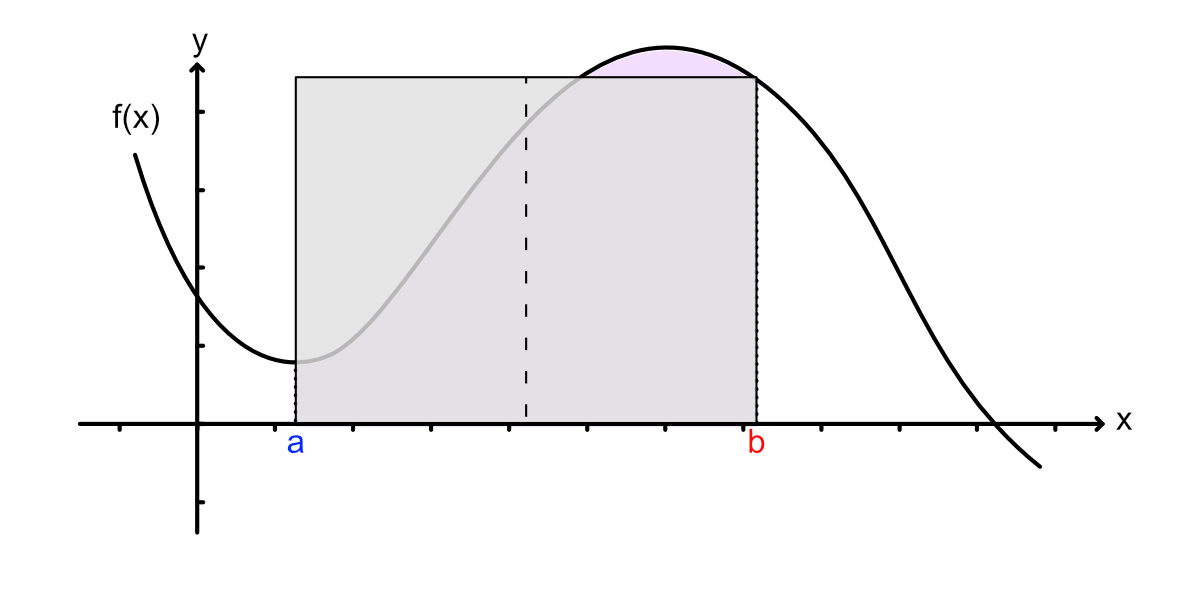
\includegraphics{grobe-approximierung-riemann.png}
\caption{Grobe Approximation}
\label{fig:grobe_approximation}
\end{figure*}

\pagebreak
Die Approximation ist noch zu grob. Durch das Unterteilen des grossen Rechteckes in viele kleine Rechtecke, kann eine bessere Approximation erreicht werden. Das Intervall $I = [a,b]$ wird in mehrere gleich grosse Teile zerlegt. Werden die Intervalle immer kleiner gemacht, so wird die Summe der Flächen der Rechtecke immer mehr an die Fläche zwischen dem Graphen und der $x$-Achse angenähert.

\begin{figure}[!h]
  \centering
  \parbox[t]{\widthof{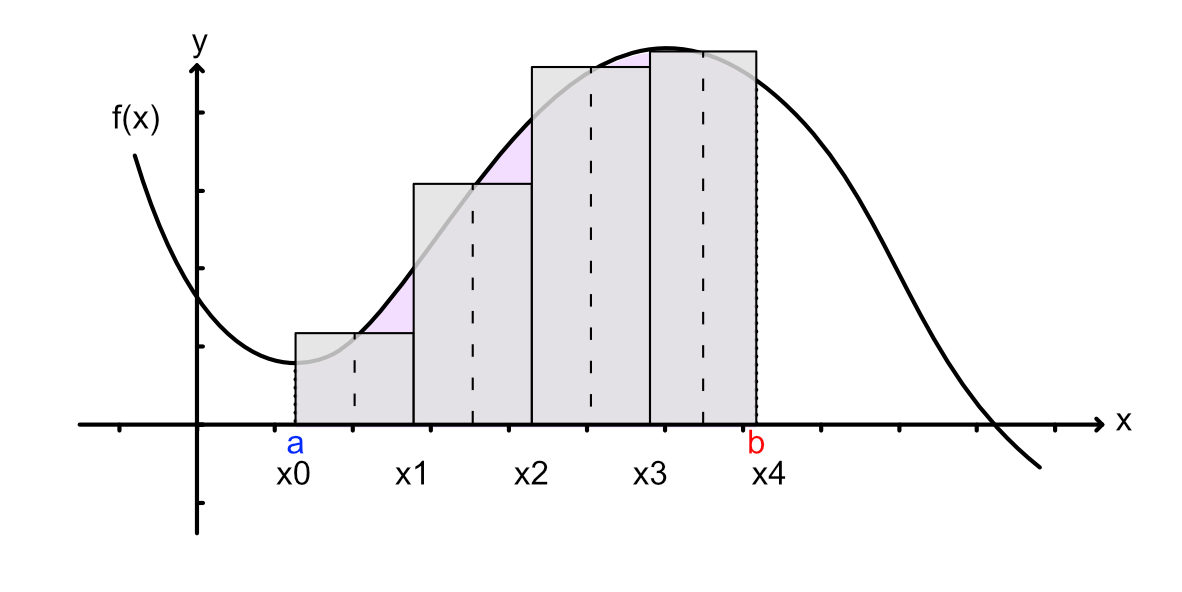
\includegraphics[width=.49\columnwidth]{mittlere-approximierung-riemann}}}{%
    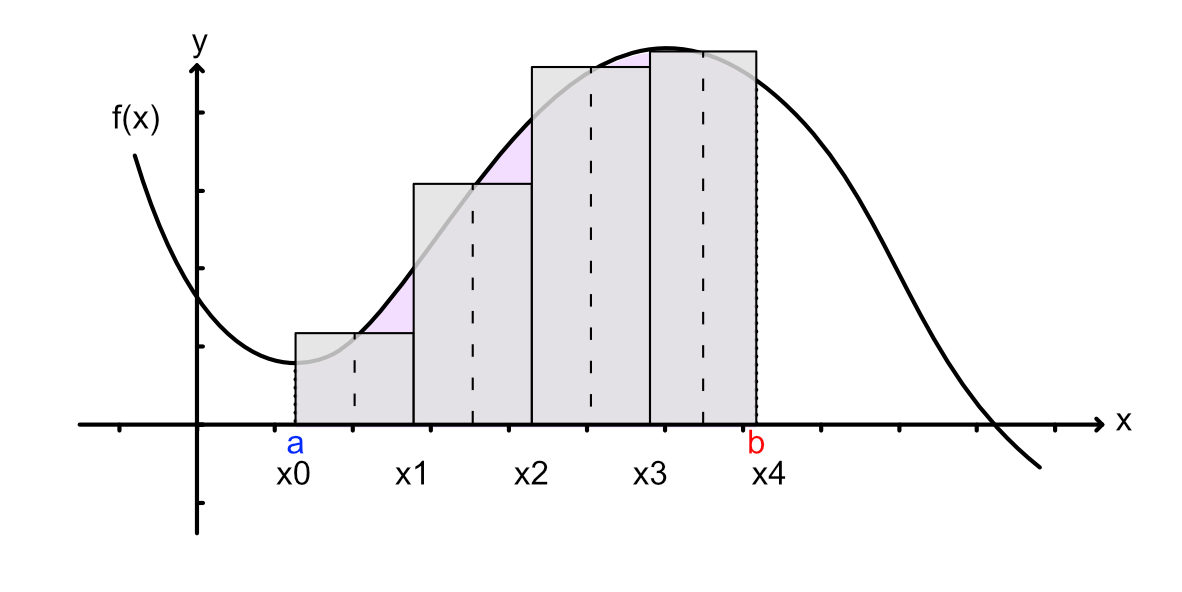
\includegraphics[width=.49\columnwidth]{mittlere-approximierung-riemann}
    \caption{Mittlere Approximation}
    \label{fig:mittlere_approximation}
  } % ein Leerzeichen Abstand
  \parbox[t]{\widthof{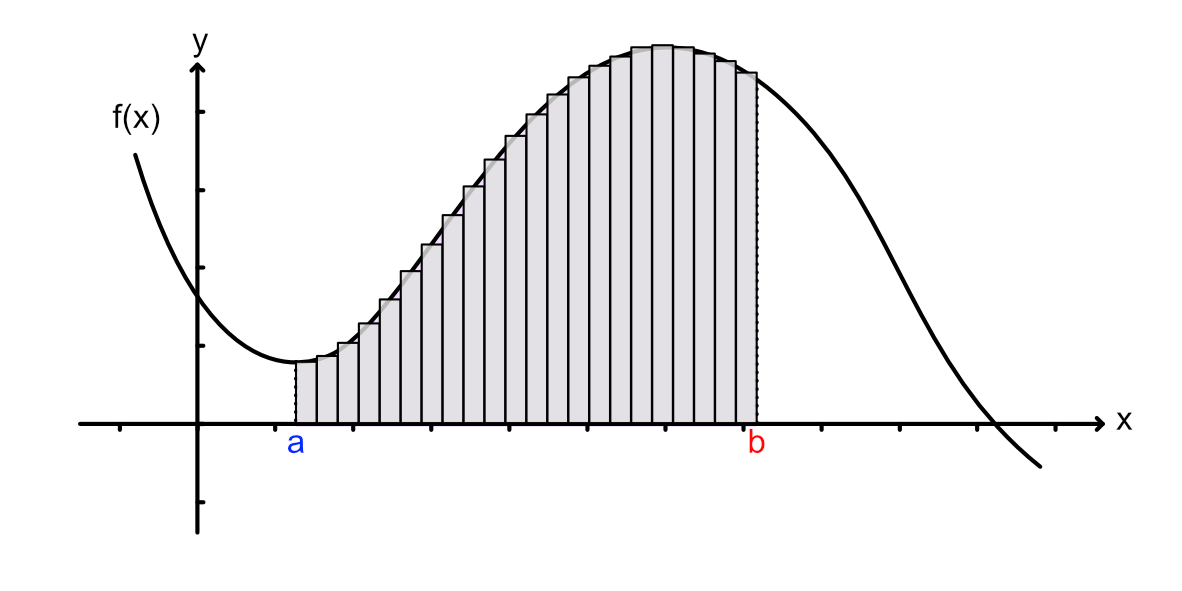
\includegraphics[width=.49\columnwidth]{feine-approximierung-riemann}}}{%}
    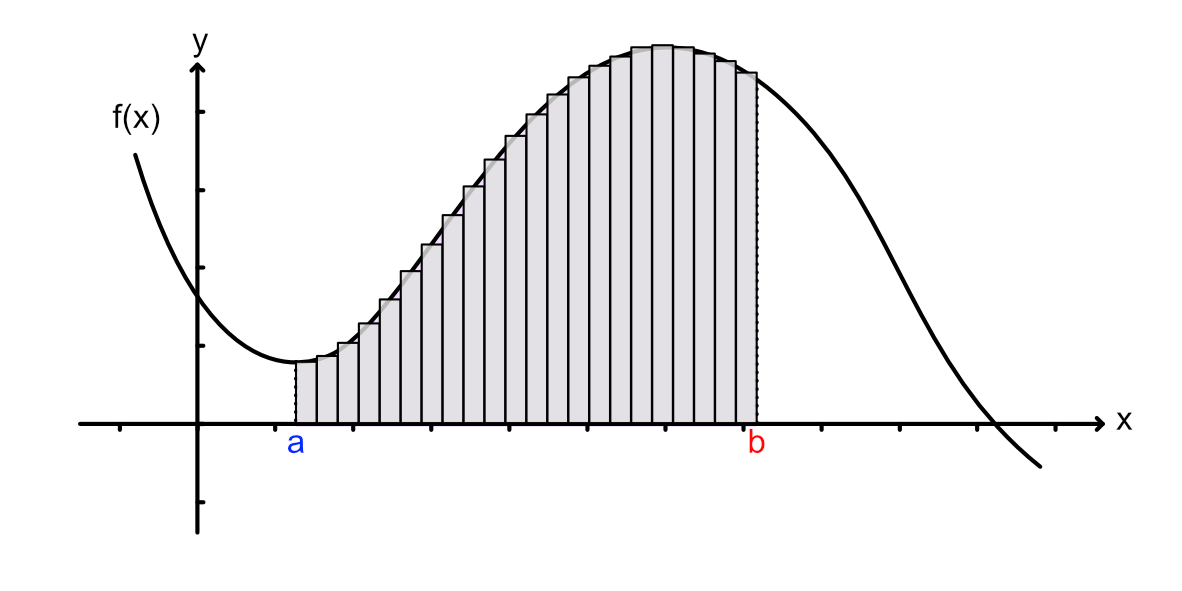
\includegraphics[width=.49\columnwidth]{feine-approximierung-riemann}
    \caption{Feine Approximierung}
    \label{fig:feine_approximierung}
  }
\end{figure}


Zählt man die Flächen der Rechtecke der mittleren Approximation aus Abbildung \ref{fig:mittlere_approximation} zusammen, erhält man eine erste Idee des Flächeninhaltes unter dem Graphen. Folgende Gleichung wird für die Fläche $F$ aufgestellt:
\[
	F = f(x)*(x_1-x_0)+f(x)*(x_2-x_1)+f(x)*(x_3-x_2)+f(x)*(x_4-x_3)
\]
Zusammengefasst wird die Summe $S$ der 4 Rechtecke wie folgt dargestellt:
\[
	S_4 = \sum_{i=1}^{4} f(x_i)\underbrace{(x_i-x_{i-1})}_{\substack \Delta x_i}
\]
Um eine grösstmögliche Approximation zu erreichen werden $n$-Rechtecke in die zu berechnende Fläche eingesetzt:
\[
	S_n = \sum_{i=1}^{n} f(x_i)\Delta x_i
\]
Diese allgemeine Form wird auch eine Riemann Summe genannt. Um den korrekten Wert für die Fläche unter dem Graphen zu erhalten, reicht eine Summe mit bestimmter Anzahl Wiederholungen nicht aus, es werden unendlich viele benötigt. $n$ muss somit nach unendlich streben:
\[
	\lim_{n\to\infty} S_n = \int_{x_0}^{x_n} f(x) dx
\]
Das gefundene bestimmte Integral nennt man das Riemann Integral. Der Wert der Funktion $f(x)$ ist dabei die Höhe des erzeugten Rechtecks, $dx$ die Breite des (unglaublich) schmalen Rechtecks.

\subsubsection{Vorgehen nach Darboux}
Ein anderes gängiges Verfahren zur Definition des bestimmten Integrals ist die Methode nach Darboux. Sie ist nach dem französischen Mathematiker Jean Gaston Darboux \cite{Darboux2020} benannt. Im Unterschied zum Riemann'schen Integral, wo die Rechtecke mittig angeordnet werden, werden die Rechtecke beim Verfahren nach Darboux unter dem Graphen minimiert oder maximiert. Passen die Rechtecke gerade noch unter die Kurve, spricht man von der Untersumme. Werden die Rechtecke so angeordnet, dass deren Höhe dem maximalen Funktionswert an dieser Position gleich ist, spricht man von der Obersumme.
\begin{figure}[!h]
  \centering
  \parbox[t]{\widthof{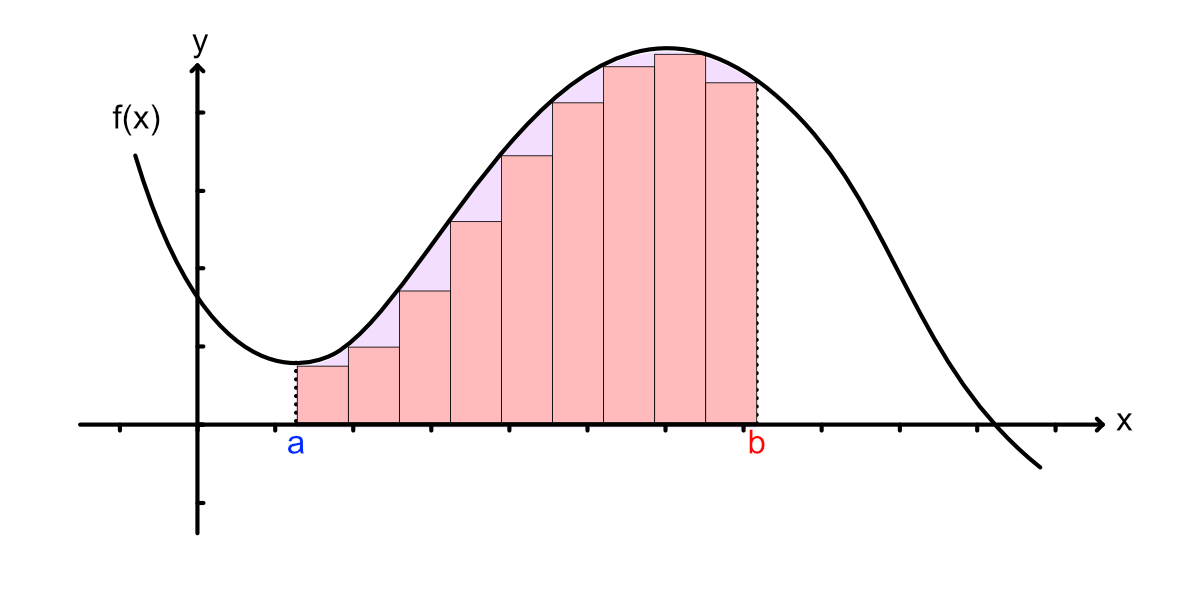
\includegraphics[width=.49\columnwidth]{untersumme}}}{%
    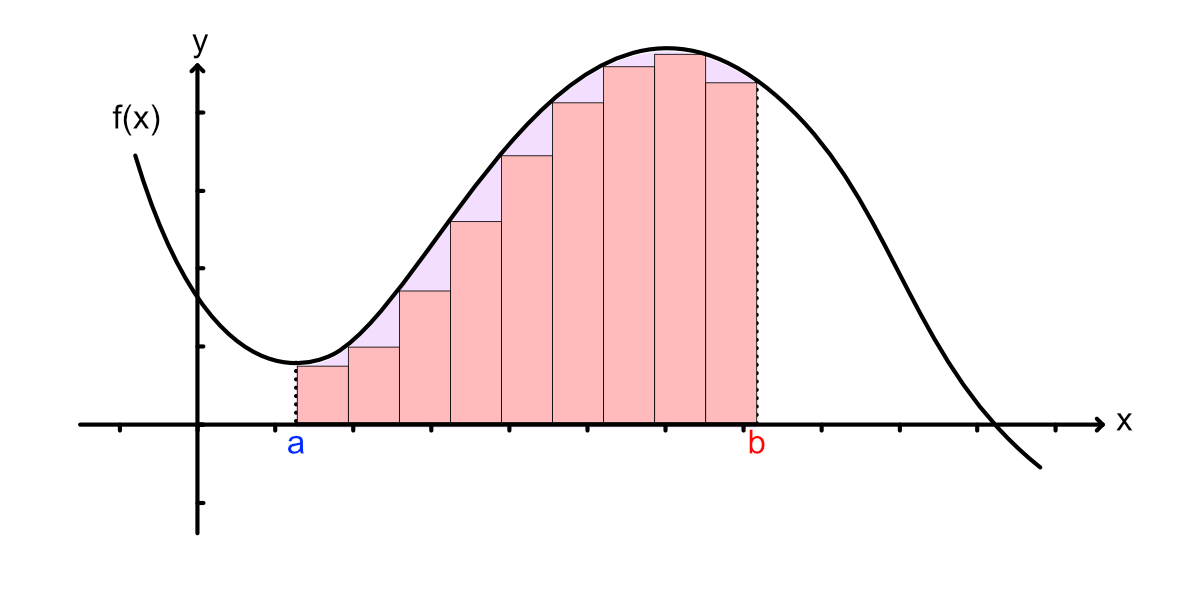
\includegraphics[width=.49\columnwidth]{untersumme}
    \caption{Rechtecke der Untersumme}
    \label{fig:untersumme}
  } % ein Leerzeichen Abstand
  \parbox[t]{\widthof{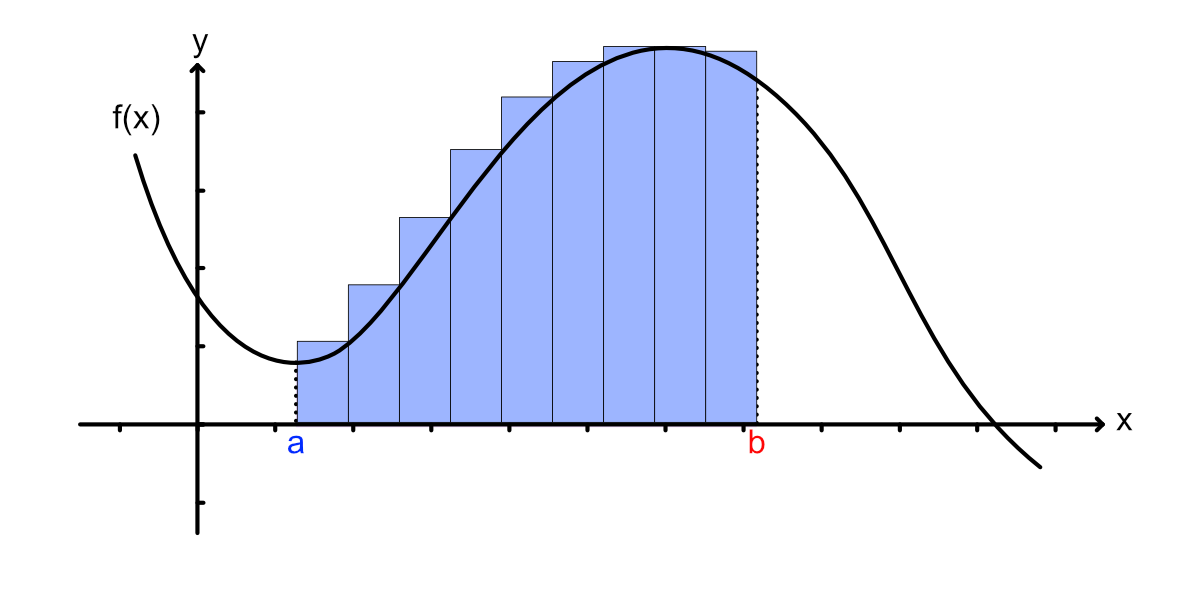
\includegraphics[width=.49\columnwidth]{obersumme}}}{%}
    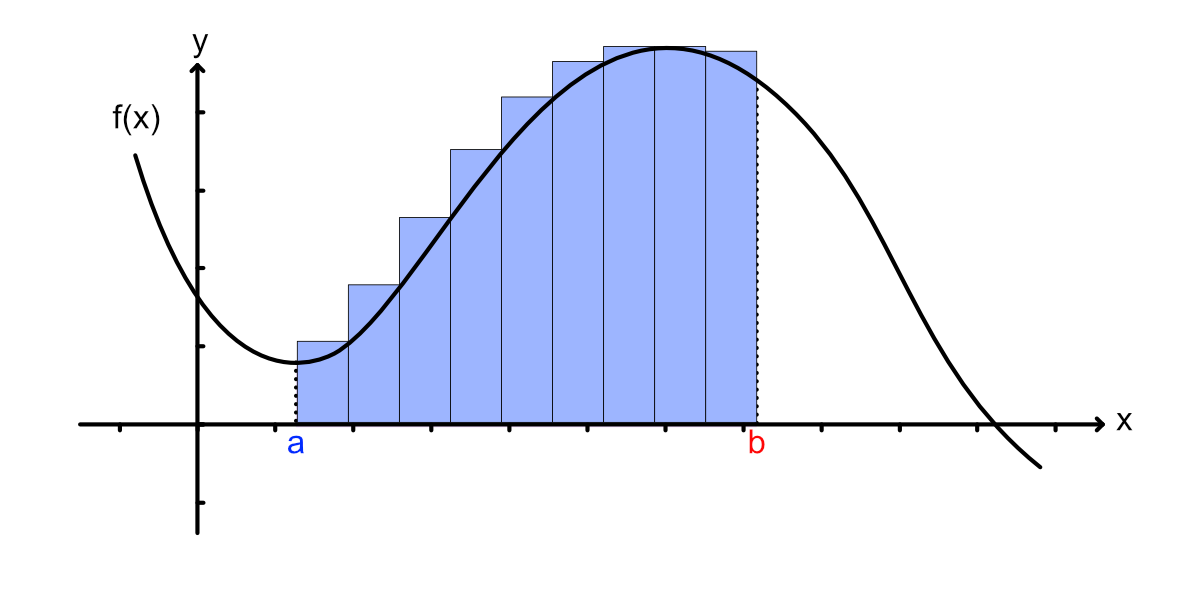
\includegraphics[width=.49\columnwidth]{obersumme}
    \caption{Rechtecke der Obersumme}
    \label{fig:obersumme}
  }
\end{figure}


%Die Folgen nähern sich für $n\rightarrow\infty$ von unten bzw. oben an den Wert des gesuchten Flächeninhaltes unter der Kurve an x.

Die Folge der Untersumme ist streng monoton wachsend. Jene der Obersumme ist streng monoton fallend \cite{Portmann2019}. Um die Unter- und Obersumme zu bilden, werden alle Flächen der Rechtecke addiert: 
\[
	U_n = A_1 +A_2+A_3+...+A_n
\]
\[
	O_n = A_1 +A_2+A_3+...+A_n
\]
Um die Folgen für die Unter- und Obersumme zu bestimmen, braucht es ein $\Delta x$. Dies bildet sich aus den Intervallgrenzen $I=[a,b]$ und der Anzahl Rechtecke $n$:
\[
	\Delta x = \frac{b -a }{n}
\]
Betrachtet man die Darstellungen für Unter- und Obersumme aus den Abbildungen \ref{fig:untersumme} und \ref{fig:obersumme} ergibt sich somit folgendes:
\[
	U_9 = \Delta x * (f(a) + f(a+ \Delta x) + f(a+ 2*\Delta x) + ... + f(a+ 8*\Delta x))
\]
\[
	O_9 = \Delta x * (f(a+ \Delta x) + f(a+ 2*\Delta x)+...+f(a+ 9*\Delta x))
\]

Zur Übersichtlichkeit wird die Formel mit einer Summenformel für die Unter- und Obersumme zusammengefasst:
\[	
	U_n = \Delta x \sum_{i=1}^{n} f(a +(i-1)\Delta x)
\]
\[
	%O_n = \sum_{i=1}^{n} f(x_i)\Delta x_i
	O_n = \Delta x \sum_{i=1}^{n} f(a+i*\Delta x)
\]
Um eine grösstmögliche Approximation für die Fläche unter dem Graphen zu erhalten, werden unendlich viele Rechtecke benötigt. $n$ muss nach unendlich streben:
\[
	\lim_{n\rightarrow\infty} U_n = \Delta x \sum_{i=1}^{n} f(a +(i-1)\Delta x)
\]	
\[
	\lim_{n\rightarrow\infty} O_n = \Delta x \sum_{i=1}^{n} f(a+i*\Delta x)
\]
 Da die Unter- und Obersumme gegeneinander zulaufen, kann die Untersumme der Obersumme gleich gesetzt werden. 
\[
	\lim_{n\rightarrow\infty} U_n =\lim_{n\rightarrow\infty} O_n = \int_a^b f(x) dx
\]
Mit der Methode nach Darboux kann ebenfalls ein bestimmtes Integral berechnet werden.


%EVENTUELL ENTFERNEN
\pagebreak
\subsection{Rechenregeln für bestimmte Integrale}
Für die bestimmten Integralen existieren die folgenden Rechenregeln.

\subsubsection{Vertauschen der Integrationsgrenzen}
Vertauscht man Untergrenze $a$ und Obergrenze $b$, ändert sich das Vorzeichen\cite{Portmann2019}.
\[
	\int_a^b f(x) dx = -\int_b^a f(x) dx
\]

\subsubsection{Obergrenze = Untergrenze}
Setzt man die Obergrenze gleich der Untergrenze ist der Flächeninhalt 0. Es existiert keine Fläche\cite{Portmann2019}.
\[
	\int_a^a f(x) dx = 0
\]

\subsubsection{Aufspalten, Zerlegen}
Ein bestimmtes Integral auf dem Intervall $[a,b]$ lässt sich in Teilintervalle aufspalten\cite{Portmann2019}.

\[
	\int_a^b f(x) dx = \int_a^c f(x) dx + \int_c^b f(x) dx 
\]

\begin{figure*}[!h]
\centering
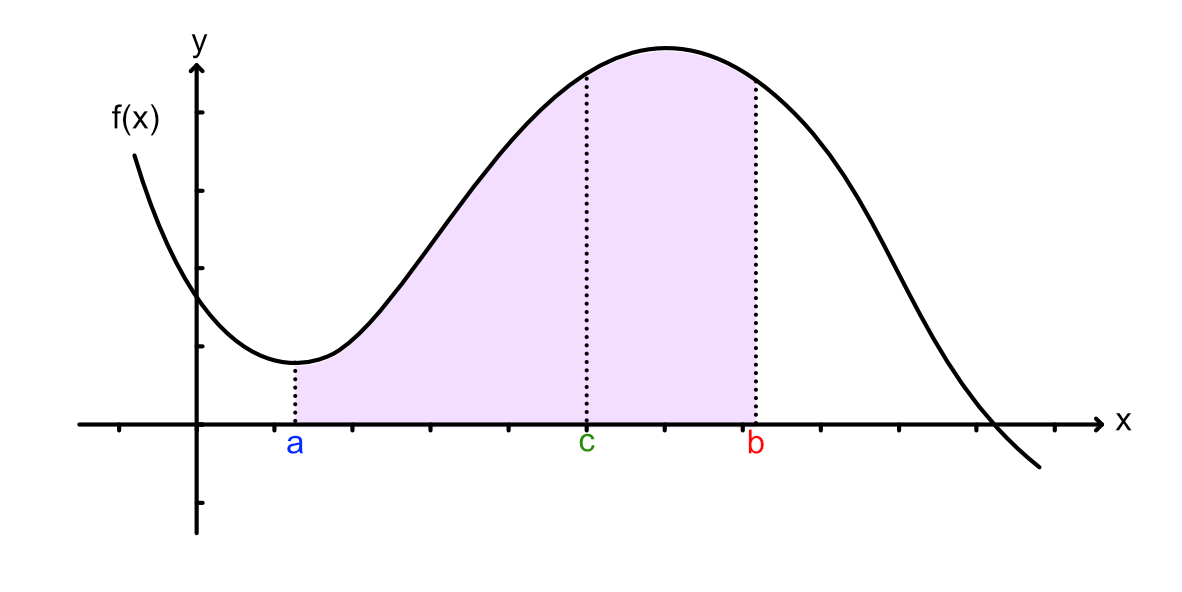
\includegraphics{intervall-teilen}
\caption{Aufteilung des Intervalls in $[a,c]$ und $[c,b]$}
\label{fig:intervall_teilen}
\end{figure*}


\clearpage
% Abschnitt fertig

\section{Beispiele und Anwendungen}
\subsection{Rechenbeispiel}
Gesucht ist die Fläche unter der Kurve der Funktion $ln(x)$ im Intervall $I=[1,6]$.

\begin{figure}[!h]
  \centering
  \parbox[t]{\widthof{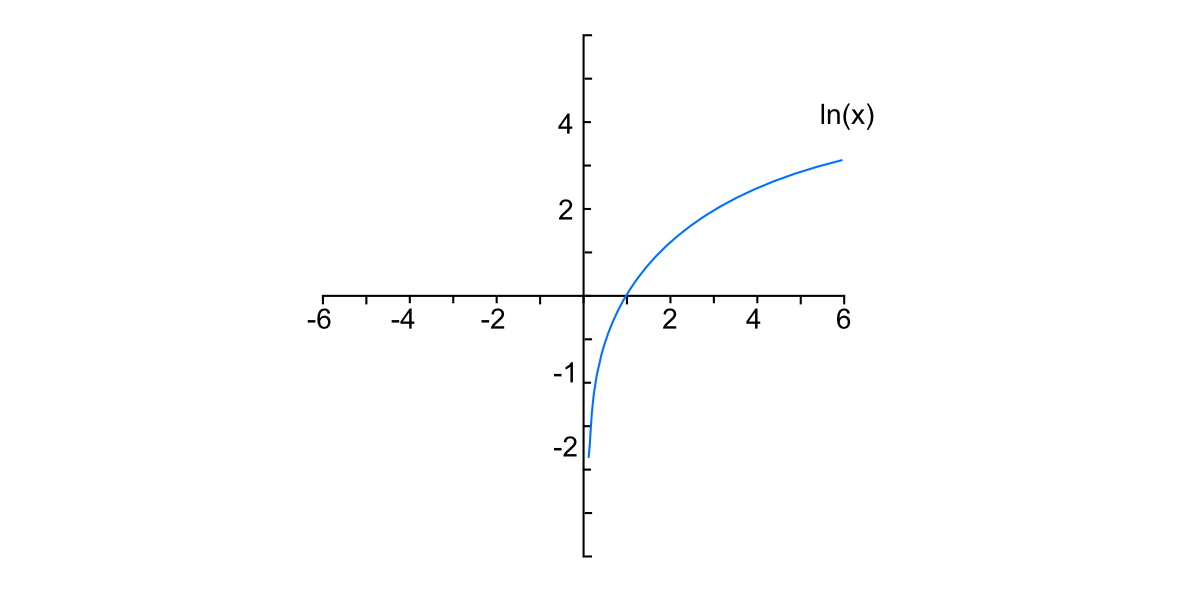
\includegraphics[width=.49\columnwidth]{rechenbeispiel-ln(x)}}}{%
    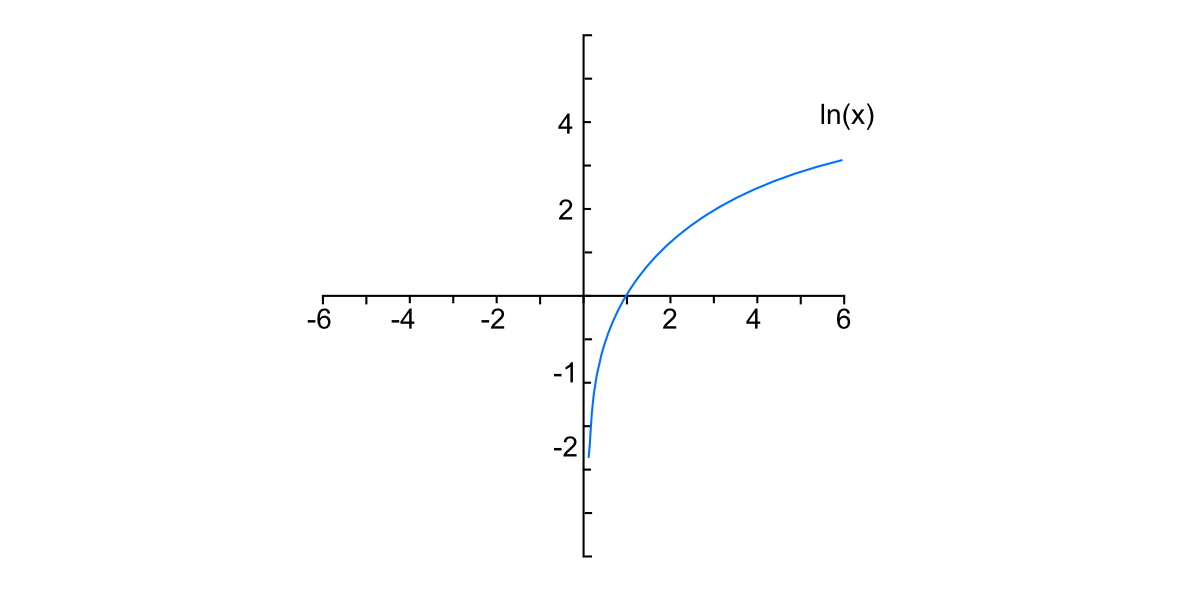
\includegraphics[width=.49\columnwidth]{rechenbeispiel-ln(x)}
    \caption{Graph der Funktion $ln(x)$}
    \label{fig:beispiel_lnx}
  } % ein Leerzeichen Abstand
  \parbox[t]{\widthof{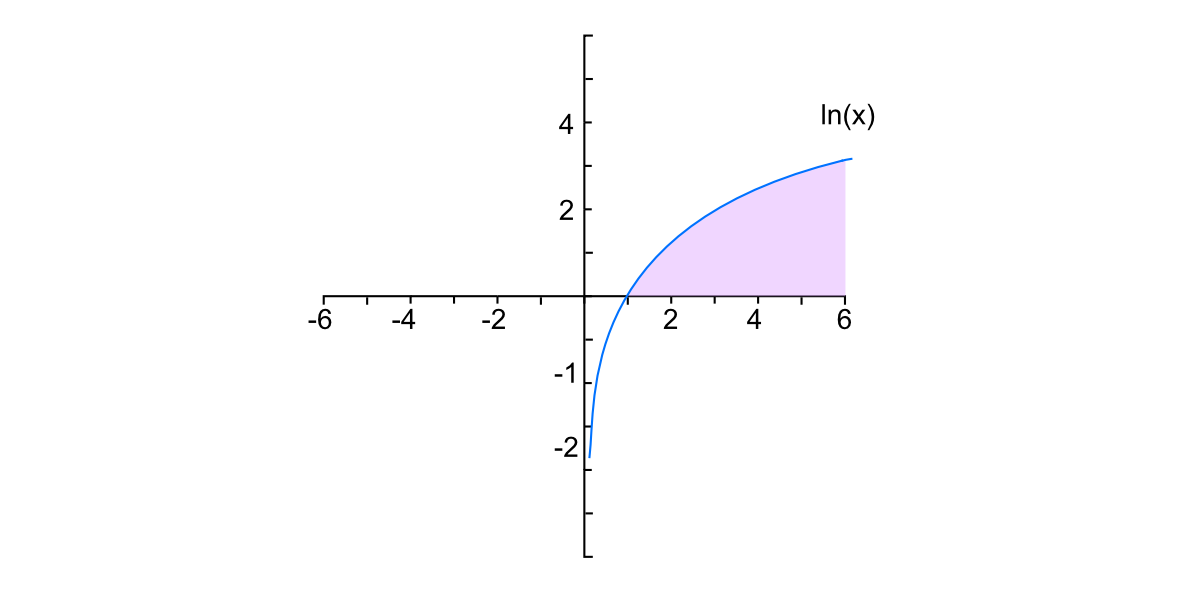
\includegraphics[width=.49\columnwidth]{rechenbeispiel-ln(x)-flaeche}}}{%}
    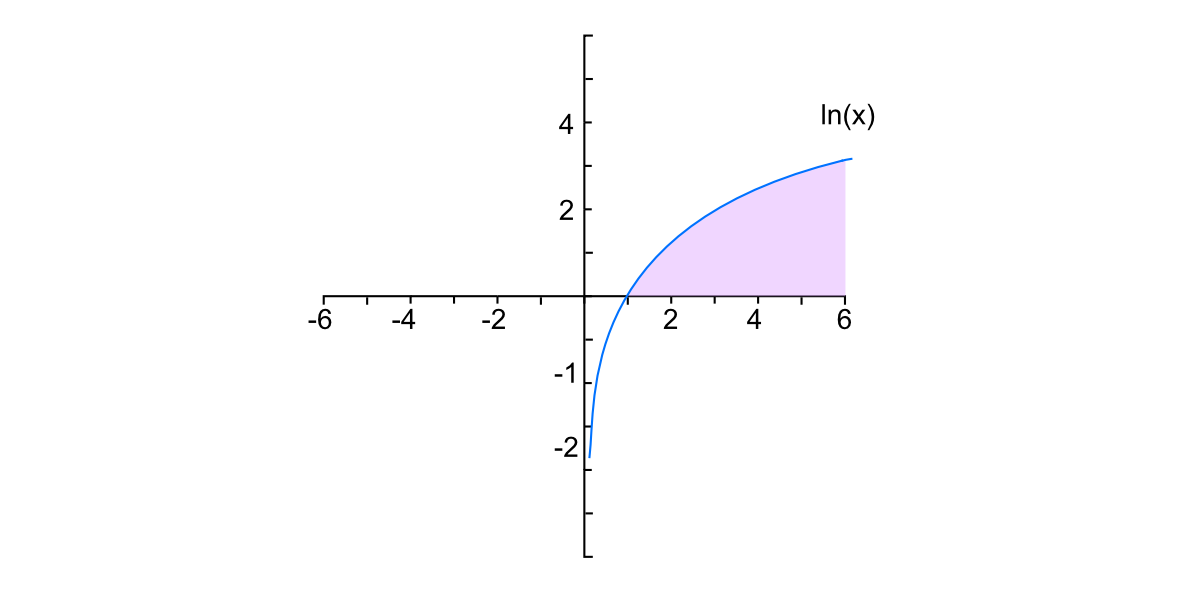
\includegraphics[width=.49\columnwidth]{rechenbeispiel-ln(x)-flaeche}
    \caption{Gesuchte Fläche unter der Funktion $ln(x)$ (violett)}
    \label{fig:beispiel_lnx_mit_flaeche}
  }
\end{figure}

Das bestimmte Integral wird wie folgt berechnet: 
\[
	\int_1^6 ln(x) dx
\]

Durch das Integrieren erhält man die Stammfunktion.

\[
	6 ln(6)-5
\]

%Ref einfügen
Die Lösung lautet $\approx 5.7506$ und entspricht der Grösse der gesuchten Fläche in Abbildung \ref{fig:beispiel_lnx_mit_flaeche}.

\subsection{Integrieren mit Python}
Das Rechenbeispiel aus Abbildung \ref{fig:beispiel_lnx_mit_flaeche} mit Python:
\begin{lstlisting}
from sympy import *
from sympy.solvers import solve
import scipy.integrate 
import numpy as np

init_printing()
x = Symbol('x')

integrate(ln(x), (x,1,6))

print("indefinite integral: %s " % integrate(ln(x), (x,1,6)))

f = lambda x: ln(x)
i = scipy.integrate.quad(f, 1,6)
print("result: %s" % i[0]) #Print only first Object as result, second is the absolute error 

Output: 
indefinite integral: -5 + 6*log(6) 
result: 5.750556815368327
\end{lstlisting}



\clearpage
% Abschnitt fertig

\bibliography{IEEEintegral}

\end{document}

